\section{Introduction and System Architecture Overview}
\label{sec:architecture}



\begin{enumerate}
    \item \textbf{Firmware Generation} (\texttt{firmware\_flow}): Automates STM32CubeMX project initialization, package installation, and code generation via CLI scripting.

    \item \textbf{AI Model Discovery and Optimization} (\texttt{ai\_flow}): Implements a two-tier model discovery system (curated task-based models + iterative web search), followed by neural network customization and hyperparameter optimization with NNI.

    \item \textbf{Firmware-AI Integration} (\texttt{integration\_flow}): Merges generated C inference code into the STM32 project structure and verifies build compatibility.

    \item \textbf{Web Research} (\texttt{search\_flow}): Provides technical guidance through RAG-improved web search with quality evaluation metrics.
\end{enumerate}

\clearpage
\begin{figure}[p]
    \centering
    \centerline{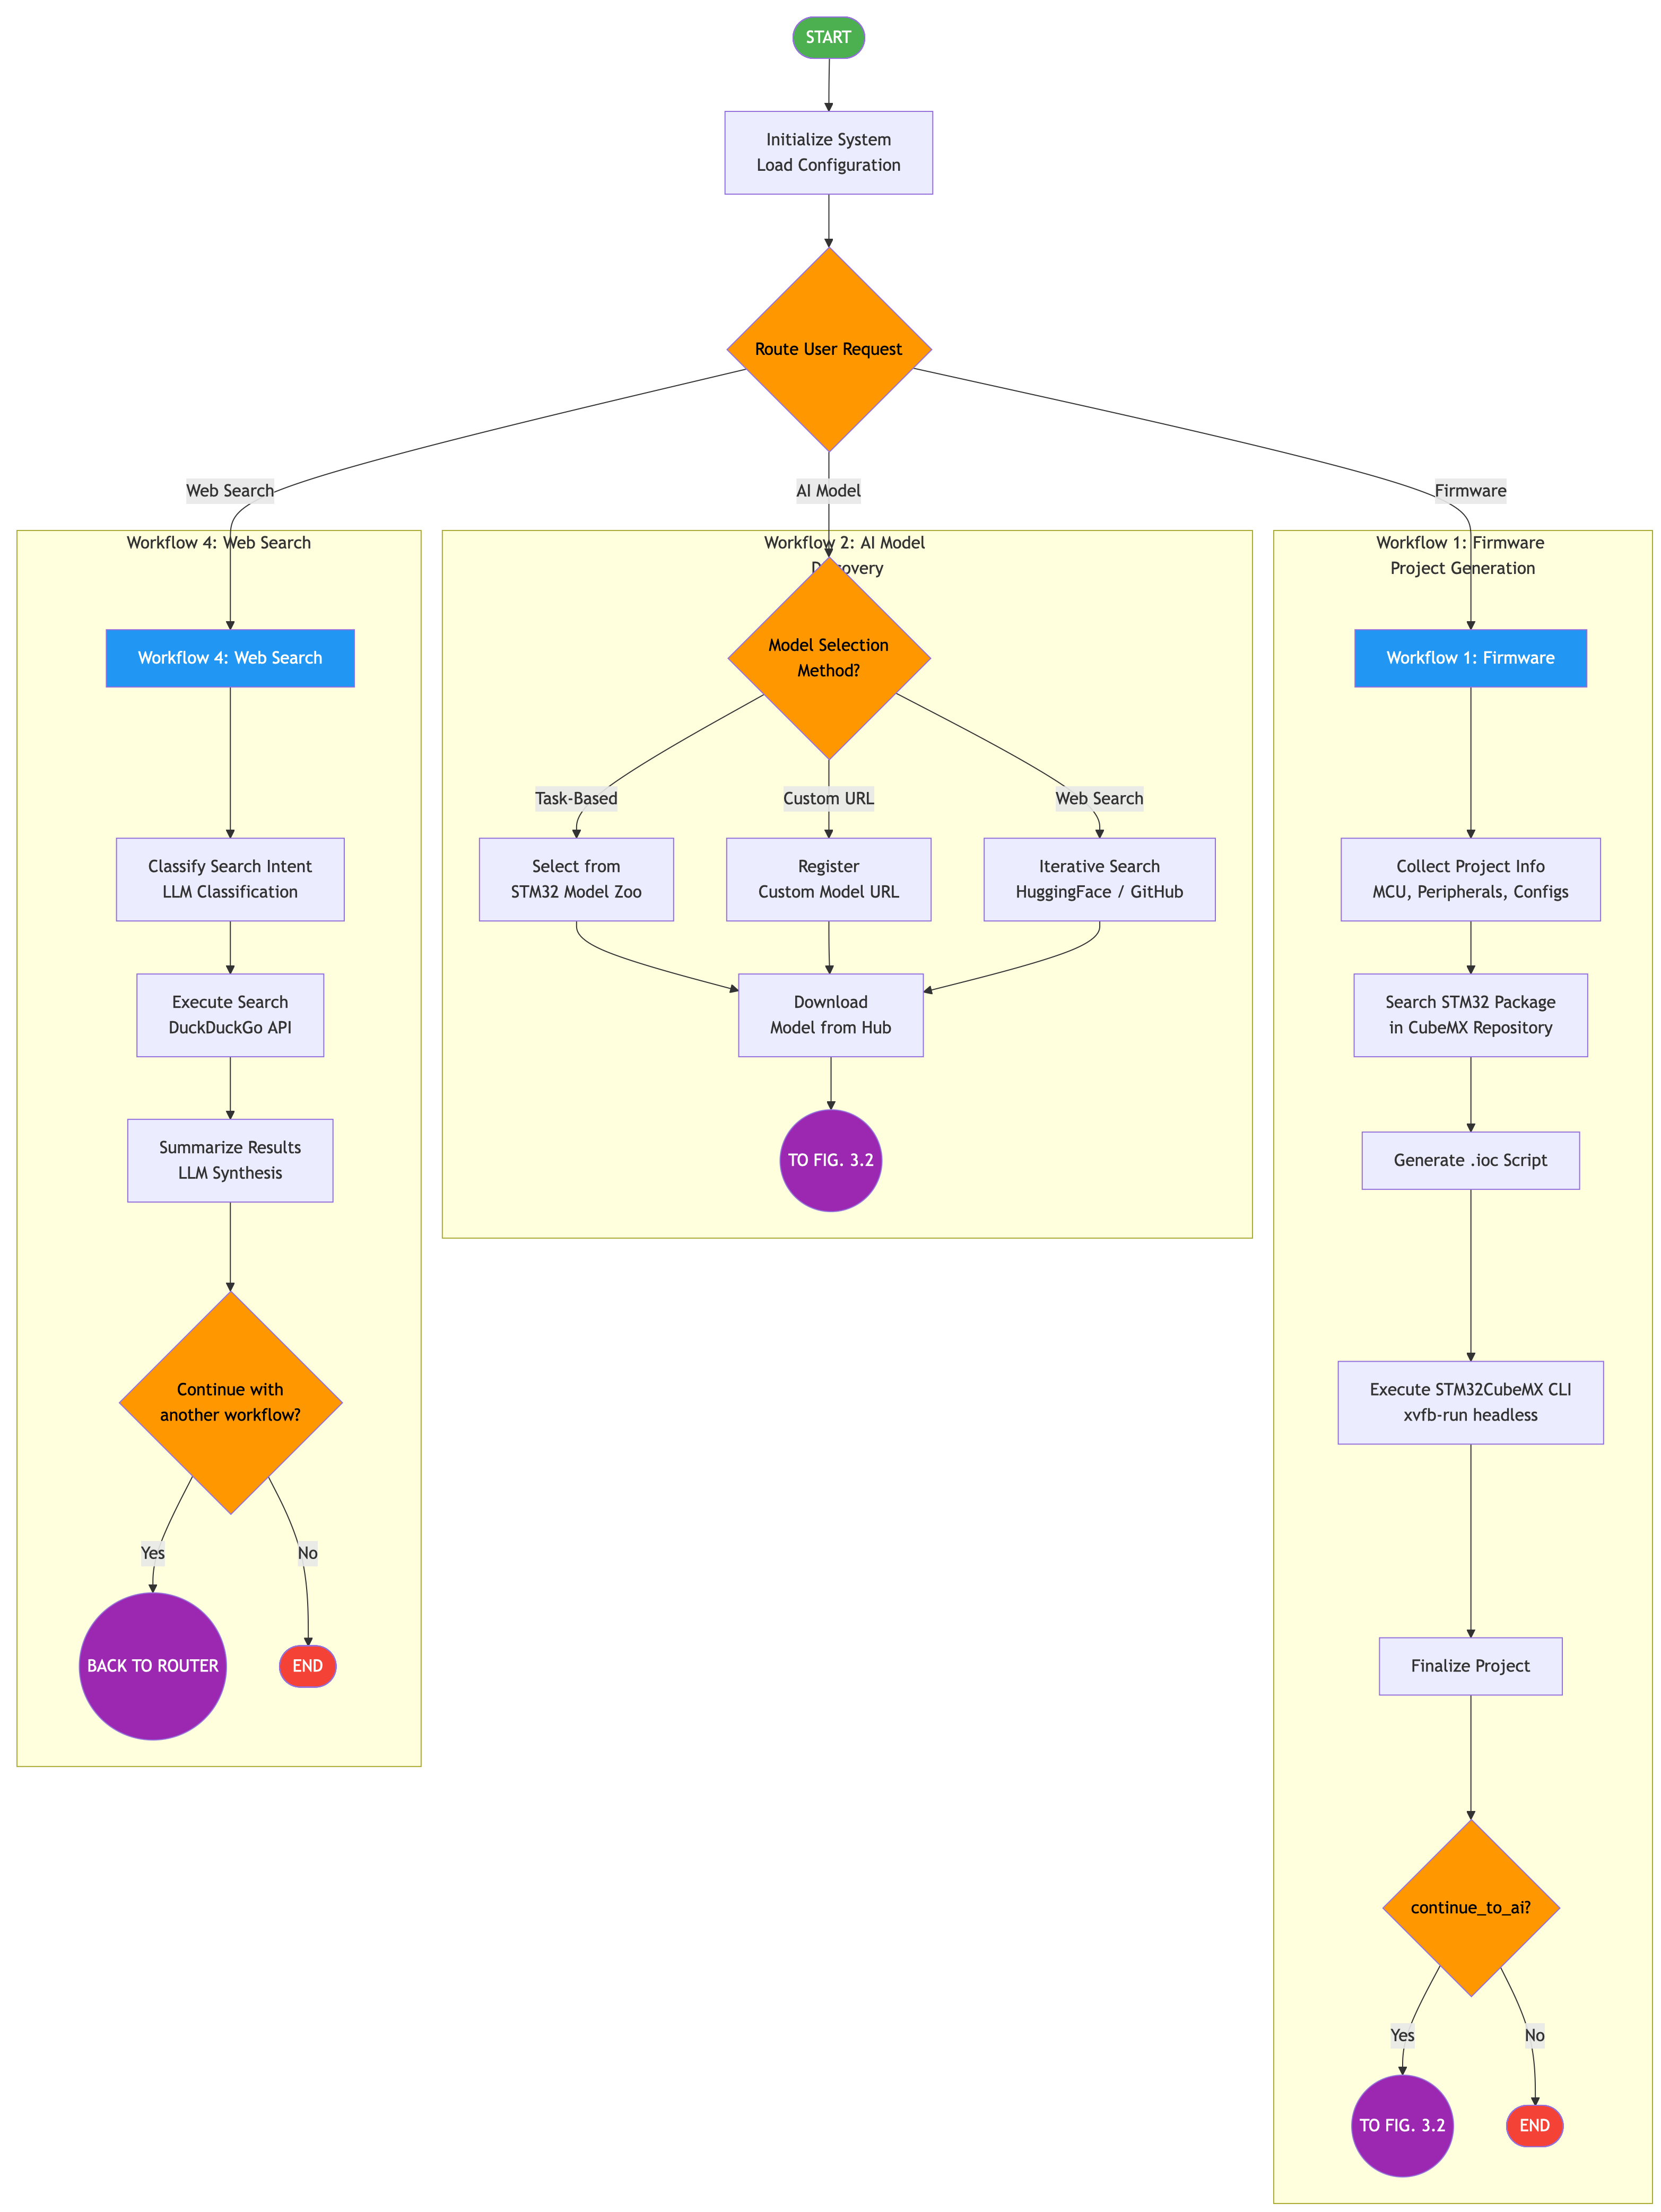
\includegraphics[width=\textwidth]{chap3/figures/part1Graph.png}}
    \caption{Global system flowchart -- Fig.~3.1: System initialization, request routing, and parallel entry workflows (Firmware Generation, AI Model Discovery, Web Search).}
    \label{fig:global_flowchart_part1}
\end{figure}
\clearpage

The routing decision is performed by an LLM-based classifier that analyzes the user's natural language input and returns a structured decision object:

\begin{lstlisting}[language=Python, caption={LLM-based routing logic from graph.py}, label={lst:routing}]
# From src/assistant/graph.py - route_request()
llm_router = ChatTriton(model="mistral").with_structured_output(RouteDecision)

result = llm_router.invoke([
    SystemMessage(content=router_instructions),
    HumanMessage(content=f"Request: {state.message}")
])

state.route = result.route  # "firmware", "ai_analysis", "integration", or "web_research"

if result.confidence < 0.6:
    logger.warning(f"Low confidence ({result.confidence:.2f}), requesting clarification")
    state.route = "unknown"
\end{lstlisting}

If the classifier's confidence falls below 0.6, the system enters a clarification loop where the user is prompted to explicitly select the desired workflow from a structured menu.

\subsubsection{State Management and Persistence}

All workflow data is stored in a single \texttt{MasterState} object defined in \texttt{state.py}. This Pydantic-based state class contains over 50 typed attributes covering:

\begin{itemize}
    \item \textbf{User Input}: Original message, intent classification, routing metadata
    \item \textbf{Firmware Workflow}: Board name, MCU series, .ioc file path, CubeMX output directory
    \item \textbf{AI Workflow}: Model path, task type, target MCU, compression level, search iteration count
    \item \textbf{Customization}: Model layers, modification parameters, NNI experiment directory
    \item \textbf{Integration}: Generated code paths, build status
    \item \textbf{Web Research}: Query history, search results, evaluation scores
\end{itemize}

This persistent state model enables \textbf{Context Chaining}, a key architectural feature where outputs from upstream workflows (e.g., the specific MCU target selected during \texttt{firmware\_flow}) automatically populate the input context for downstream workflows (\texttt{ai\_flow}). This eliminates redundant user data entry and prevents configuration mismatches, such as selecting an AI model incompatible with the previously generated firmware board. The state object acts as a \textit{single source of truth}, synchronizing project parameters across heterogeneous toolchains (CubeMX, STEdgeAI, TensorFlow).

LangGraph automatically persists this state at every node transition through a checkpointing mechanism, enabling:

\begin{enumerate}
    \item \textbf{Fault Tolerance}: Resume execution from the last successful checkpoint after transient failures
    \item \textbf{Human-in-the-Loop Gates}: Suspend execution for user approval without losing context
    \item \textbf{Time-Travel Debugging}: Replay past executions to diagnose workflow errors
\end{enumerate}

A detailed analysis of the underlying storage infrastructure and the dual-layer memory management logic is provided in Section \ref{sec:redis_architecture}.

\subsubsection{Robustness in LLM-Driven Orchestration}

Relying on Large Language Models for orchestration decisions introduces non-determinism. During stress testing with concurrent users, unconstrained LLM outputs occasionally caused validation crashes or incorrect routing. The framework solves this by enforcing three layers of input normalization before any LLM response modifies the \texttt{MasterState}.

First, I implemented type coercion for numerical parameters. When extracting data like sample rates for synthetic data generation, LLMs frequently append human-readable units (e.g., \textit{``2 kHz''} instead of \texttt{2000}). The framework preemptively normalizes these strings into raw floating-point measurements before passing them to Pydantic, bypassing strict validation errors.

Second, I introduced regex-based fallbacks for hardware identification. If the LLM extracts an imprecisely formatted identifier (hallucinating prefixes like \textit{``STM32 F401''} instead of \texttt{STM32F401}), a relaxed regular expression (such as \texttt{r'(?:STM32)?[\textbackslash{}s-]*([A-Z])([0-9])'}) guarantees the core MCU series letter and digit are captured correctly for the downstream ST toolchains.

Finally, I adopted an enumerated prompt anchoring strategy. During model discovery, providing the LLM with only the total count of available models resulted in hallucinated index selections when users specified model names. Injecting the complete, enumerated list of model names directly into the extraction prompt creates a bounded decision space and enforces deterministic routing.

\subsubsection{System Integrity and Transactional Registration}

To maintain the stability of the model registry, the framework implements a \textbf{Transactional Registration Flow} for user-provided models. When a user submits a new model URL, the entry is first held in a \textit{Pending} state within the \texttt{MasterState}. The system then performs an autonomous validation via the STEdgeAI analysis engine. Only upon successful technical profiling (\texttt{analyze\_success = true}) is the model permanently committed to the \texttt{predefined\_models.json} registry. This transactional behavior ensures that the system's knowledge base remains free from broken links, malformed architectures, or incompatible file formats.

\subsection{Configuration Management}

Runtime parameters are managed through a dedicated \texttt{Configuration} class (\texttt{configuration.\allowbreak py}) that dynamically loads settings from a prioritized hierarchy of sources. \textbf{Environment Variables} are used for sensitive data such as STMicroelectronics credentials (\texttt{ST\_EMAIL}, \texttt{ST\_PASSWORD}) and API keys, while a local \textbf{Config File} (\texttt{config.json}) defines system-specific paths including the STM32CubeMX binary location, the STM32Cube repository path, and AI output directories. 

In addition, the \textbf{LangGraph Runtime Config} enables the injection of per-request settings directly into each workflow node via the \texttt{config} parameter.

The framework relies on several important parameters to govern its behavior: \texttt{local\_llm} defines the language model identifier (defaulting to \texttt{mistral:latest}), while \texttt{llm\_temperature} balances deterministic routing ($0.0$) with creative code generation ($0.2$). The \texttt{llm\_\allowbreak context\_\allowbreak window} manages token limits, typically $4096$--$8192$, and \texttt{cubemx\_path} points to the absolute location of the STM32CubeMX CLI. 

For AI-specific workflows, the \texttt{ai\_target} specifies the target MCU (e.g., \texttt{stm32h743}), and \texttt{ai\_compression} sets the desired quantization level ranging from \texttt{low} to \texttt{very\_high}. All parameters are validated at runtime using \textbf{Pydantic validators}, to ensure that required paths exist and credentials are correctly formatted before the orchestrator starts any workflow execution.

\subsection{Graph Topology and Node Composition}

Each of the four primary workflows is implemented as a \textbf{subgraph} with its own internal routing logic. The master graph connects these subgraphs through conditional edges that allow \textit{inter-workflow transitions} based on user decisions:

\begin{itemize}
    \item After completing firmware generation, the system offers to proceed to AI model discovery
    \item After AI model optimization, the system offers to integrate the generated C code into the firmware project
    \item At any point, users can invoke web research to gather technical documentation
\end{itemize}

This multi-stage pipeline mirrors the typical embedded AI development lifecycle:

\begin{center}
    \texttt{Hardware Setup → Model Selection → Model Customization → Code Generation → Integration → Testing}
\end{center}

The graph construction logic resides in four primary "injection" functions:

\begin{itemize}
    \item \texttt{inject\_\allowbreak firmware\_\allowbreak nodes()}: Firmware workflow (Workflow 1)
    \item \texttt{inject\_\allowbreak ai\_\allowbreak analysis\_\allowbreak nodes()}: AI discovery, customization, and data management (Workflows 2, 5, 6, 7)
    \item \texttt{inject\_\allowbreak integration\_\allowbreak nodes()}: Firmware-AI integration and verification (Workflow 3)
    \item \texttt{inject\_\allowbreak web\_\allowbreak search\_\allowbreak nodes()}: Web research and RAG support (Workflow 4)
\end{itemize}

Each function encapsulates the node definitions and internal routing logic for its respective domain, adding them to the master \texttt{StateGraph} builder.

\clearpage
\begin{figure}[p]
    \centering
    \centerline{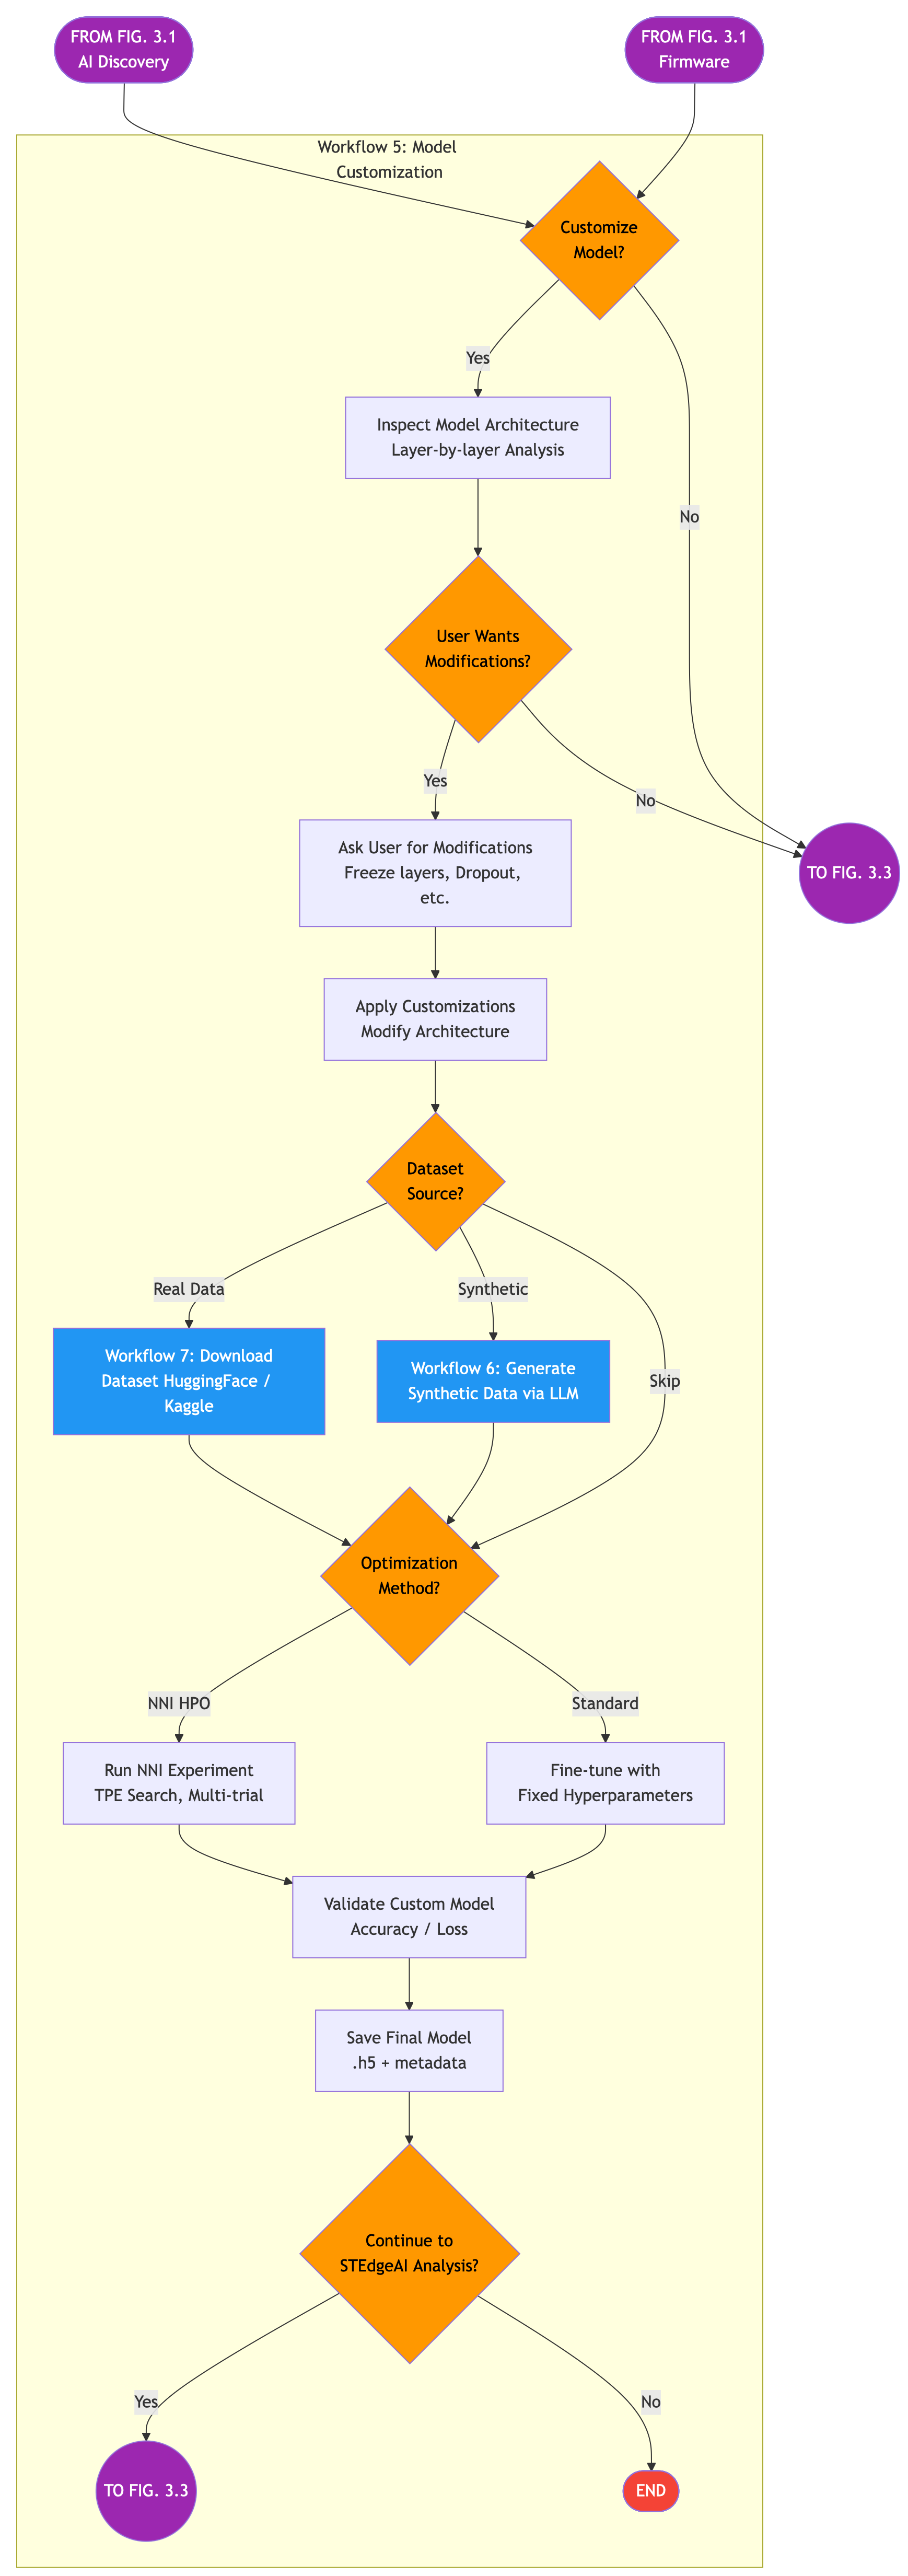
\includegraphics[height=0.9\textheight]{chap3/figures/part2.png}}
    \caption{Global system flowchart -- Fig.~3.2: Model customization workflow (Workflow~5), including architecture inspection, dataset acquisition, and hyperparameter optimization via NNI.}
    \label{fig:global_flowchart_part2}
\end{figure}
\clearpage

\clearpage
\begin{figure}[p]
    \centering
    \centerline{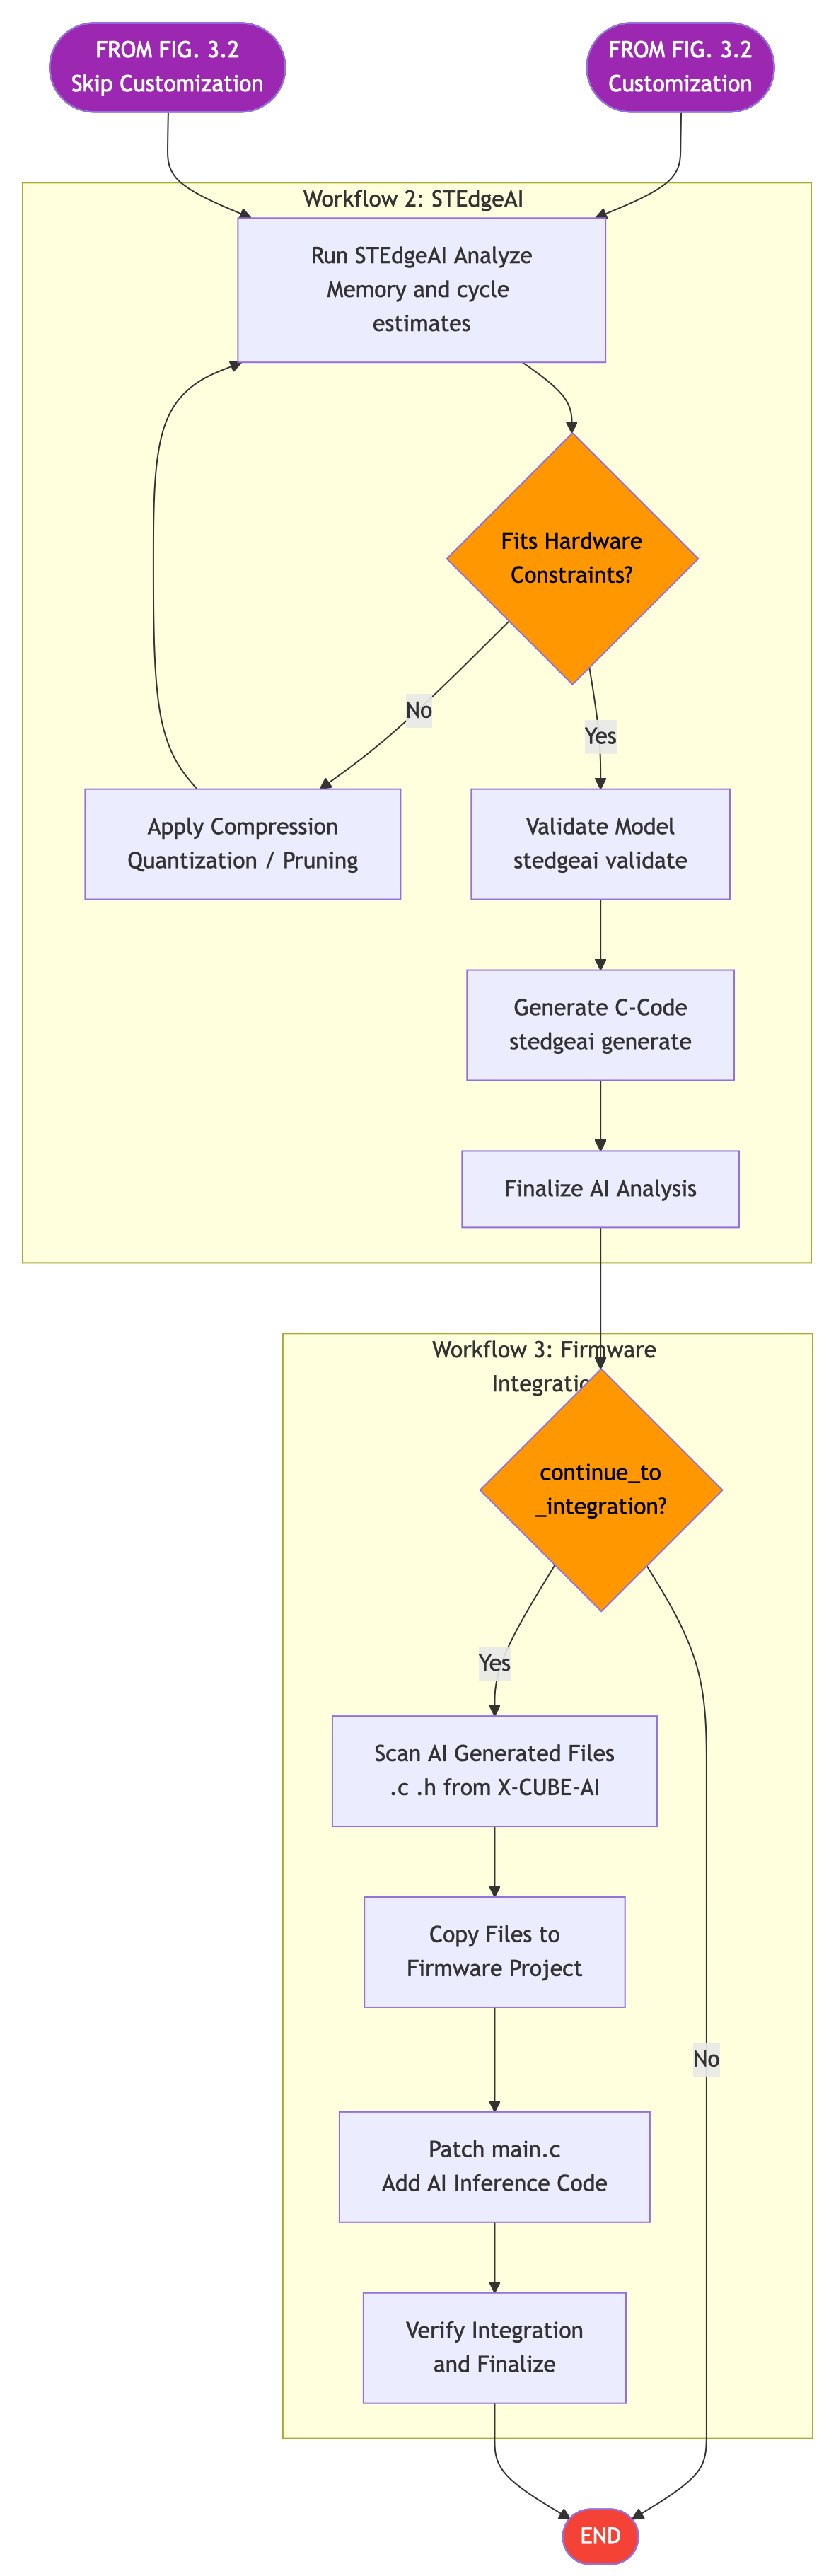
\includegraphics[height=0.9\textheight]{chap3/figures/part3.png}}
    \caption{Global system flowchart -- Fig.~3.3: STEdgeAI analysis loop, C-code generation, and firmware integration workflow (Workflows~2 and~3).}
    \label{fig:global_flowchart_part3}
\end{figure}
\clearpage

\subsection{Logging and Observability}

The system implements a multi-tier observability strategy, combining structured backend logging with real-time progress streaming. Technical logs are managed via the standard Python \texttt{logging} library with distinct severity levels.

\textbf{DEBUG} logs provide detailed execution traces, including LLM prompt-response pairs and internal state transitions, while \textbf{INFO} logs track high-level operational events such as workflow entry, node completion, and subprocess execution. \textbf{WARNING} logs are reserved for non-fatal anomalies, such as low LLM confidence scores or active fallback mechanisms, and \textbf{ERROR} logs capture recoverable failures, including API timeouts or malformed user inputs requiring re-interaction.

A specific architectural feature is the log interception mechanism: logs generated by critical nodes, such as training status or hardware configuration, are captured by a dedicated \texttt{QueueHandler} and streamed to the client using the \textbf{Newline Delimited JSON (NDJSON)} format. This allows frontend clients, such as the \textit{Gradio UI} or the \textbf{VS Code extension}, to provide immediate status visualization and progress bars, transforming a complex multi-step backend process into a transparent and interactive user experience.


